\chapter{Preparation}
This project involved vast exploratory design work, in preparation of the actual implementation.

	\section{Requirements}
	This project could go in numerous different design directions from the start. Since the functionality and its benefits over existing systems depended heavily on the design chosen, it was hard to separate what benefits the program would achieve from what features the program would include and how it would expose them to the user. 
	
	However, in order to focus our exploration and make sure that the focus was on achieving some real deliverables for end users, a requirement analysis was necessary. The following functional goals were listed based on the project proposal, which focus on what basic tasks the system must help the user achieve, while allowing leeway in how the program exposed and implemented these features.
	
	The system must allow the user to:
	\begin{enumerate}[label=\bfseries Core \arabic*:]
		\item Use any data they have in reasonably arranged formats in common file types.
		\item Specify the type of chart they want by drawing a likeness of it on screen using a stylus.
		\item Bind the data to the chart using an interface that makes it clear how the data is affecting the visualisation.
		\item Specify visual, size and positioning properties of the chart through the sketches.
		\item Manipulate the visual appearance of the created chart.
	\end{enumerate}
	
	In addition, time permitting, the system may:
	\begin{enumerate}[label=\bfseries Extension \arabic*:]
		\item Transform user-drawn sketches to show the visual link to the formal chart elements.
		\item Feed back manipulations applied to the formal layer back to the user drawn sketches, in order to keep the visuals of the formal and sketch layers in synchronisation.
		\item Allow users to undo actions by erasing sketches, and remove the corresponding formal elements without throwing errors.
		\item Allow users to manipulate any property of chart elements, not just one, so that the domain of visualisations they can create is infinite. For example, allow them to bind not just the height of bars in a bar chart to data, but also their width and colour. 
		\item Analyse the data and infer properties that may allow it to automatically suggest properties of the chart, such as which field belongs on which axis, or whether a data series should be log scale or linear scale.
		\item The user must be able to export the chart as a Microsoft Chart object that can be embedded as a dynamic object in Microsoft Office files, not just as a raster image.
	\end{enumerate}
	
	The core of this project focusses on making more usable software, rather than providing additional functionality, compared to existing systems. Hence, some usability goals were also specified:
	\begin{enumerate}[label=\bfseries Usability \arabic*:]
		\item Users must be able to create charts at least as quickly as they can using current systems.
		\item Users must be able to build a mental model of the software's behaviour within 2 uses of it. They should thus be able to accurately predict the consequences of any action taken within the software.
		\item Changes to the information visualisation must occur through directly manipulating the visual representation of the chart, rather than through disconnected User Interface widgets.
		\item The user must be able to easily try out changes to the visualisation, see what that would look like, and undo them if needed.
	\end{enumerate}
	
	\section{Design Goals}
	In order to meet the usability requirements, some design principles need to be followed. The main benefit of a sketch-based interface is that it is more likely to match the user's mental model, or their expectation of what every UI widget will do, since it draws upon familiar metaphors, and offers liveness and direct manipulation of the visualisation. This section explores the theories of direct manipulation and liveness, and how they might be applied to this project.
	
	\begin{quote}
	Direct manipulation systems offer the satisfying experience of operating on visible objects. The computer becomes transparent, and users can concentrate on their tasks. [It] permits novice users access to powerful facilities without the burden of learning to use a complex syntax and lengthy list of commands. Direct manipulation involves three interrelated techniques: 
		\begin{enumerate}
			\item Provide a physically direct way of moving a cursor or manipulating the objects of interest.
			\item Present a concrete visual representation of the objects of interest and immediately change the view to reflect operations.
			\item Avoid using a command language and depend on operations applied to the cognitive model which is shown on the display.
		\end{enumerate}			
	\end{quote}
	%TODO cite
	\begin{flushright}
	\citep{shneiderman_direct_1983}
	\end{flushright}
	
	``Liveness in programming environments generally refers to the ability to modify a running program. Liveness is one form of a more general class of behaviors by a programming environment that provide information to programmers about what they are constructing.'' \citep{tanimoto_perspective_2013}
	
	\section{Work Items}

	The following broad work items were identified as necessary to achieve the objectives above:
	%TODO Maybe insert a picture of my development process here, including the user studies?
	\begin{enumerate}
		\item Get the requisite approvals for the human study from the Ethics Review Committee.
		\item Assess the various methods to build a classifier for ink recognition, including using the RATA Framework.
		\item Run an initial user study to  see how people naturally draw graphs, and also use it to collect training examples for the classifier.
		\item Build a UI that accepts strokes, runs them through the classifier, and shows the user feedback to indicate successful recognition.
		\item Build the UI widget that lets users import their spreadsheets in Microsoft Excel (xlsx) or Comma Separated Value (csv) files. It must then expose the various fields detected.
		\item Build the charting component to convert the recognised sketches and the ink into a finished visualisation.
		\item Run a pilot study followed by a user study to evaluate the system.
	\end{enumerate}	
	
	An iterative development process, similar to the Spiral Model and Scrum, was adopted for this project. This allowed early experimentation with and user testing of the various components and different interface designs. After each iteration of the code development, we came across design decisions that needed to be made. After evaluating the various options, we would build one out, resulting in a new iteration, and then repeat the process.
	
	To manage technical debt and follow best practices, we adopted a form of Test-Driven Development (TDD). In its pure form, TDD relies on a fully planned out functional specification and automated testing. However, since the design and functionality of this project were evolving over time, small specifications were made for each iteration, and changed as necessary after a sprint (to borrow Scrum terminology). Also, since the input needed to sketched by hand, and the output was visual and changes in literal pixel values between trials, it was non-trivial to simulate and verify this interaction automatically. These parts were verified through repeated manual testing each time the code was changed or refactored. Parts of the code that were effectively in a functional programming style (deterministic calculations with no side effects) could, however, be checked with unit tests. In addition, to pick up design flaws early, the prototypes were constantly used for hallway testing (friends and family were asked to use the application and speak out what they were thinking as they did).
	
	Thanks to the constant refactoring of the code to minimise coupling, the project could be open sourced at the end and plugged in as a standard GUI component in other Windows applications in the end, making sure that this software can actually be used.
	
	
	
	
	
	\section{Development Environment}
	For this project, the hardware available was a Microsoft Surface Pro (\nth{1} gen), which features the active digitizer screen required for precise inking. Since this machine runs Windows by default, we chose to develop the system using the .NET framework, which has built-in support for Tablet PCs and Ink handling.
	
	As a precaution, insurance was taken out on the machine to ensure quick replacement in case of damage or loss. Additionally, version control was used extensively in the project, to ensure no work was lost. The code for the RATA ink stroke recogniser, described below, was uploaded to a Git repository in collaboration with RATA's authors. The code for this project was then written in a fork of that repository, to allow updates to RATA to be pulled in. The dissertation itself was written in \LaTeX , so that the text files could be versioned in another Git repository. Both repositories were backed up off-site on repository host Bitbucket. The dissertation was also backed up online using file synchronisation software Microsoft OneDrive. 
	
	\section{Building the classifier}	
	Core to the system is an ink recognition component that identifies the chart element (e.g.\ bar, axis) that the user has sketched. This must work above a certain accuracy threshold or the system will prove frustrating to users \citep{frankish_recognition_1995}. However, since the project scope included other components too, the time available to build this classifier was limited. Additionally, given the complexity of building a classifier, and our limited experience with building them, it would be difficult to get the same accuracy as those provided in a mature library. Hence, we decided to build a classifier using existing tools rather than implementing one from scratch. 
	
	\subsection{Recognition Method}
	A number of different approaches have been taken in building systems that automatically interpret hand-drawn sketches. These approaches vary in the recognition accuracy they offer, and the robustness to generalise across multiple domains. \citep{ouyang_visual_2009}. Some of the approaches that have been attempted:
	
	\begin{itemize}
		\item Focus on \textbf{defining shapes structurally}. A base vocabulary of primitives like lines, ellipses and arcs is built by describing the properties of such shapes. \citep{shilman_statistical_2002} used a hand-coded grammar to describe shapes in a domain as a composition of such primitives. \citep{alvarado_sketchread:_2004} used dynamically constructed Bayesian networks to scale this process to multiple domains. \citep{hammond_ladder:_2006} developed a language to manually describe how diagrams in a domain are drawn, displayed and edited. 
		\item Look at the \textbf{visual appearance} of shapes and symbols. \citep{kara_image-based_2004} used image-based similarity metrics to perform template matching. \citep{shilman_recognition_2004} broke up the ink into connected subgraphs of nearby strokes, which were then compared to known symbols. \citep{oltmans_envisioning_2007} proposed a visual parts-based method that utilise a library of shape contexts to describe and identify symbols in a domain.
		\item \textbf{Compute features} of the ink. \citep{patel_ink_2007} selects these features and sets their thresholds statistically. \citep{yu_domain-independent_2003} uses heuristics for the same purpose. \citep{chang_rata._2010,  rubine_specifying_1991, willems_iconic_2009} all use machine learning to automatically find relationships between features and choose an appropriate feature set accordingly.
	\end{itemize}		
	
	\citep{chang_rata._2010} showed that the first two approaches forego some accuracy, since they rely on the final pixel values of the sketch and so do not fully exploit the rich temporal data stored with digital ink. Within the last approach, they showed that using machine learning allows recognisers to be generated for new domains with less effort than statistical or heuristic methods. Since the domain for this charting application could grow over time, we wanted a recogniser that could be adapted easily over time. Using data mining, this can be done using training data rather than programming effort.
	
	Having decided on using a feature-based approach that selects the feature set by data mining a training dataset, there were a number of alternatives available to us. While most projects, like \citep{rubine_specifying_1991} and \citep{willems_iconic_2009}, rely on one or two data mining algorithms, \citep{chang_rata._2010}'s RATA.SSR combines the results from four well-performing algorithms in WEKA \citep{hall_weka_2009} tuned to their best configurations, to provide a more accurate recogniser. RATA.SSR thus outperformed all the other recognisers tested (PaleoSketch \citep{paulson_paleosketch:_2008}, CALI \citep{fonseca_cali:_2002}, \$1 recogniser \citep{wobbrock_gestures_2007}) on domains other than the one they were explicitly demonstrated on. 
	
	Besides, RATA.SSR also has the advantaged of outputting an API that can be plugged into our system after we build the recogniser. Additionally, one of the authors, Beryl Plimmer, previously worked with some members of the Graphics and Interaction Group at the Cambridge Computer Laboratory, and so could be reached for support and source code, which proved to be an invaluable resource.
	
	\subsection{Data collection}
	After acquiring RATA, we inspected the code and did manual testing, which revealed some blocking bugs. Since we were in contact with the authors of the software, we were able to confirm with them that these were indeed bugs. We implemented fixes for them and contributed them back to the authors, and are working towards getting the code ready for to be published Open Source.
	
	With a working version of RATA, an initial study was run to collect training data. We asked 10 participants (20-26 year old Cambridge students, studying a large variety of subjects) to draw a chart. I spoke out the following prompt:
	
	\begin{quotation}
	Imagine you are a government official trying to use a bar chart to visualise how the population has grown over time. Can you sketch out what this bar chart might look like? Just treat this screen like paper.
	\end{quotation}
	
	 They were then presented a simple UI with a large white canvas and the following task description written in a panel:
	
	\begin{quotation}
	Draw 2 axes. Label the x axis 'Year' and the y 'Population'. Draw 3 bars of different heights. Each shape (axis, bar) should be drawn in one stroke.
	\end{quotation}
	
%	First, they were shown a spreadsheet file containing sample data as below:
%	\begin{tabu}{l r r}
%		\rowfont{\bfseries} Year & Births & Deaths \\
%		2010 & 50,000 & 30,000 \\
%		2011 & 40,000 & 35,000 \\
%		2012 & 36,000 & 37,000 \\
%		2013 & 34,000 & 35,000 \\
%	\end{tabu}
%	
%	\vspace{10pt}
%	
%	Next, I spoke out the following task prompt.
%
%	
%	\begin{quote}
%		Say you are a government official trying to visualise trends in birth and death rates over time. Could you draw a bar hart on this screen that you would need to visualise this. No need to plot the actual data, just a rough sketch of what this chart would look like.	
%	\end{quote}
	
	They were asked to draw the same chart 2 times, in order to get 20 training samples in total, and to observe how much variation there is between multiple sketches by the same user. On the second drawing, they were encouraged to draw a less conventional chart, to make the system as robust in the face of variations as possible. 
	%TODO ^Explain this better
		
	\begin{figure}[h]
        \centering
        \begin{subfigure}[b]{0.5\textwidth}
                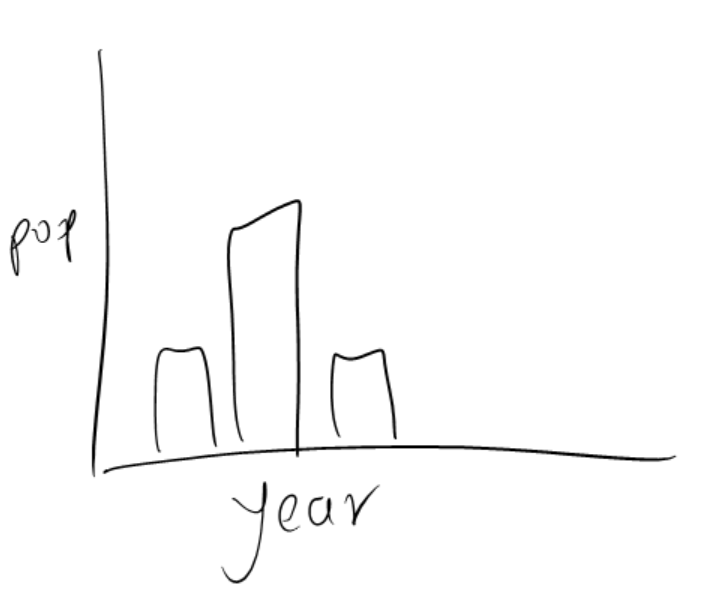
\includegraphics[width=\textwidth]{collection1}
                \caption{Regular chart}
                \label{fig:regular}
        \end{subfigure}%
        ~ %add desired spacing between images, e. g. ~, \quad, \qquad etc.
          %(or a blank line to force the subfigure onto a new line)
        \begin{subfigure}[b]{0.5\textwidth}
                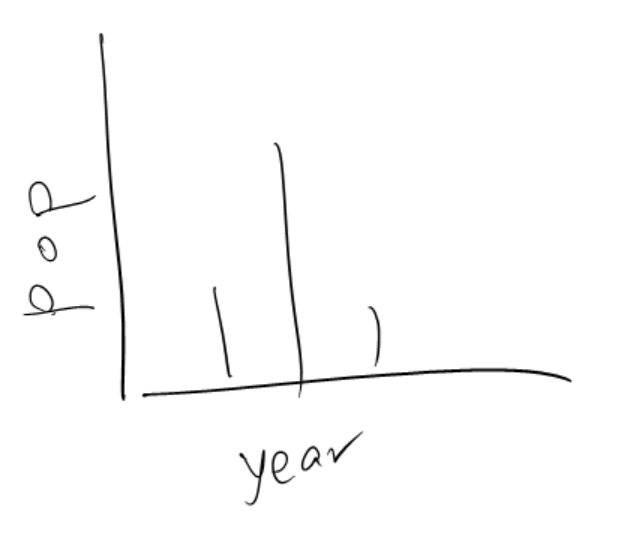
\includegraphics[width=\textwidth]{collection2}
                \caption{Using lines instead of bars}
                \label{fig:lines}
        \end{subfigure}
        ~ %add desired spacing between images, e. g. ~, \quad, \qquad etc.
          %(or a blank line to force the subfigure onto a new line)
          \begin{subfigure}[b]{0.5\textwidth}
                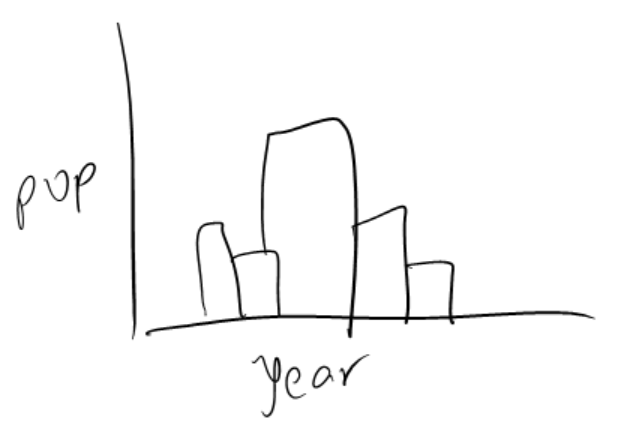
\includegraphics[width=\textwidth]{collection3}
                \caption{Grouped bars}
                \label{fig:grouped}
        \end{subfigure}%
        ~ %add desired spacing between images, e. g. ~, \quad, \qquad etc.
          %(or a blank line to force the subfigure onto a new line)
        \begin{subfigure}[b]{0.5\textwidth}
                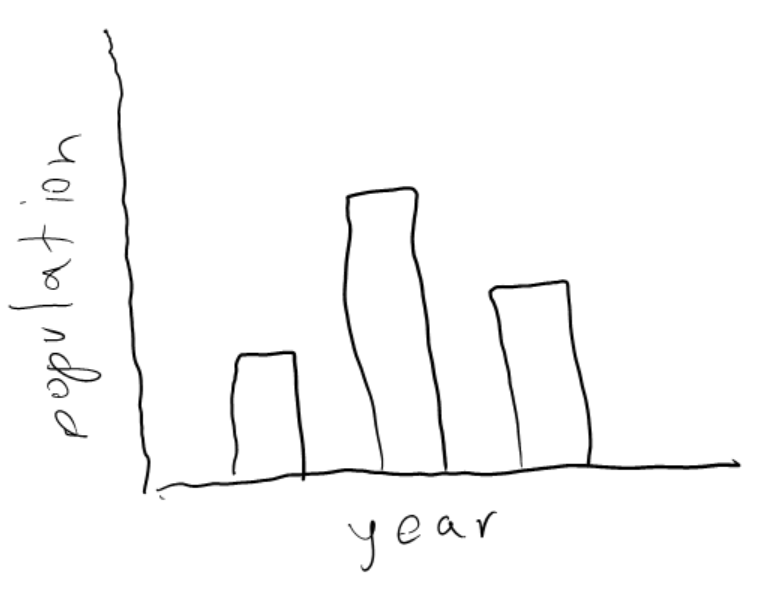
\includegraphics[width=\textwidth]{collection4}
                \caption{Using a mouse instead of the stylus}
                \label{fig:trembling}
        \end{subfigure}
        ~ %add desired spacing between images, e. g. ~, \quad, \qquad etc.
          %(or a blank line to force the subfigure onto a new line)
        \caption{Some of the more unusual chart sketches collected}\label{fig:data_collection_samples}
	\end{figure}
	
	Three elements were then defined: Axis, Bar and Text (an extra element, 'L Axis' was added later based on feedback from a pilot user study). We went through each figure and labelled the various elements.
	
	\begin{figure}[h]
		\centering
		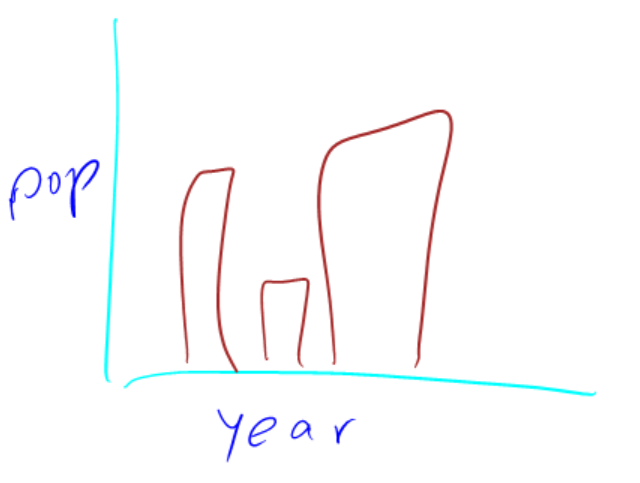
\includegraphics[width=0.5\textwidth]{collection_labelled}
		\caption{Elements of the sketch labelled as Axis (cyan), Bar (brown) or Text (dark blue)}
		\label{fig:collection_labelled}
	\end{figure}

	Once all the elements in all the charts were labelled, we could begin training. RATA includes a dataset generator tool that allowed easy extraction of various features of the strokes, such as 'distance from first to last point', 'absolute curve of largest segment' and 'pressure variation'. Data for 121 such attributes, about 270 ink strokes was compiled into a .csv file for use in training. 
	\subsection{Training}	
	The labelled data was then sent to a 'Vote' classifier in Weka, which combines the probability distributions derived from multiple classifiers \citep{kuncheva_combining_2004}. Specifically, the types of classifiers combined were Logit Boost, Bayes Net, LMT (Logistic Model Trees) and Random Forest. In order to assess how well each of these individual classifiers were performing, an experiment was set up using Weka Experimenter. The data collected in the initial study was shuffled, and then 66\% was chosen randomly as training data, the rest as testing. Then a paired T Test gave the following results:
	
	%TODO Make this all stay together as much as possible.

\vspace{10pt}
Tester:     Paired Corrected T Tester

Analysing:  Percent correct

Confidence: 0.05 (two tailed)

%\begin{table}[thb]
%
%%\scriptsize
%{\centering
%\begin{tabular}{c p{0.9 \textwidth}}\\
%(1) & meta.LogitBoost '-P 100 -F 0 -R 1 -L -1.7976931348623157E308 -H 1.0 -S 1 -I 10 -W trees.DecisionStump' 8627452775249625582 \\
%(2) & bayes.BayesNet '-D -Q bayes.net.search.local.TAN -- -S BAYES -E bayes.net.estimate.SimpleEstimator -- -A 0.5' 746037443258775954 \\
%(3) & trees.LMT '-P -I 50 -M 200 -W 0.0 -A' -1113212459618104943 \\
%(4) & trees.RandomForest '-I 100 -K 0 -S 1' -2260823972777004705 \\
%\end{tabular}
%}
%\caption{\label{}Classifier Algorithms Used}
%\end{table}

%\begin{table}[h]

%\footnotesize
%{\centering \begin{tabular}{lrr@{\hspace{0.1cm}}cr@{\hspace{0.1cm}}cr@{\hspace{0.1cm}}c}
%\\
%\hline
%Dataset & LogitBoost & BayesNet & & LMT & & RandomForest & \\
%\hline
%Initial study & 97.05 & 98.15 &         & 98.80 &         & 96.07 &        \\
%\hline
%\multicolumn{8}{c}{$\circ$, $\bullet$ statistically significant improvement or degradation}\\
%\end{tabular}  \par}
%\caption{\label{}Comparison of accuracy of the algorithms used}
%\end{table}


\begin{table}[h]
\centering
\begin{tabular}{l c}
\textbf{Algorithm} & \textbf{Accuracy} \\
LogitBoost 	&	97.05 \\
BayesNet 	&	98.15 \\
LMT			&	98.80 \\
RandomForest &	96.07 \\

\end{tabular}
\caption{Comparison of accuracy of the algorithms used}
\end{table}




